\section{Numerical Experiments}\label{sec:experiments}

\subsection{Introductive example: Quantitative Trait Loci and Association Mapping}


Many quantitative traits in plants and animals are heritable.  When
considering Mendelian traits a single polymorphic section of DNA (the
Quantitative Trait Locus) explains a significant fraction of the
phenotypic variability. However many traits are subject to the control
of several genes. These associated genes
 may prove difficult to find because of their limited individual effect.  

Yield or tasseling time of corn is typically a complex trait whose
heritability is explained by more than one gene. A possible method for
mapping association between trait and Genotype consists in regressing
the phenotype of interest  against the genotype using penalized regression.

In this introductive example, we considered a Maize Association
Mapping Panel described in \citep{RincentEtAl2014} where 269
individuals were genotyped with a 50k SNPs array. After classical data
cleaning, we kept 261 individuals and 29849 markers (SNPs).


We tested two different implementations of Lasso for selecting markers
explaining tasseling time: \mytexttt{glmnet} \citep[Generalized Linear
Models regularized by Lasso and elastic-NET,][]{2009_JSS_Friedman} and
our own implementation, by resolution of the worst-case quadratic
problem, which is shipped within an \mytexttt{R} package
\mytexttt{quadrupen} publicly available at the second author's web
page\footnote{or directly at
  \mytexttt{\href{http://stat.genopole.cnrs.fr/logiciels/quadrupen}}. This
  will be made available on the CRAN (Comprehensive R Archive
  Network)}.


The two implementation defaults were used and the optimal penalty selected by leave one out. \mytexttt{glmnet} selected 169 markers among the 29849 SNPs whereas \mytexttt{quadrupen} selected only a subset of 156 markers. 

Where does this $10\%$ difference in the number of QTL comes from since there is theoritically one unique solution to our convex Lasso problem ? 

In the following we argue  that \mytexttt{glmnet} precision is highly affected by the threshold controling the stopping condition. A first hint ....




\subsection{Synthetic data}

This section compares the performances of our algorithm to its state-of-the-art
competitors from an optimization viewpoint.  Efficiency may then be assessed by
accuracy and speed:  accuracy is the difference between the optimum of the
objective function and its value at the solution returned by the algorithm;
speed is the computing time required for returning this solution.
Obviously, the timing of two algorithms/packages has to be compared at similar
precision requirements, which are rather crude in statistical learning, far from
machine precision \citep{Bottou08}.

We compare the performance of the proposed quadratic solver with
representatives of the most successful competing algorithms.
First, we use our own implementations of all competitors, so as to provide
comparisons without implementation biases (language, library, etc.).
We use \mytexttt{R} with most of the matrix calculus done in \mytexttt{C++} using
the \mytexttt{RcppArmadillo} package \citep{2011_JSS_rcpp,armadillo} that relies
on \mytexttt{BLAS/LAPACK} libraries for linear algebra operations.
Second, we compare our code to the leading standalone packages that are
available today, so as to provide comparisons avoiding a possible competence
bias.

We use simulated data to obtain representative average results. 
Their generation covers the typical attributes of the real data encountered in
post genomic and signal processing.
In these domains, the main optimization difficulties result from
ill-conditioning, which is either due to the high correlation between
predictors, or to underdetermination when the number of variables
exceeds the sample 
\iflong 
  size (also known as the high-dimensional or the ``large $p$ small $n$'' 
  setup).
\else
  size.
\fi
For the optimization algorithms based on active set strategies, bad
conditioning is somehow alleviated when the objective function has a regular
behavior when restricted to the subspace containing the solution.  All other
things being equal, this local conditioning is thus governed by the
sparsity of the unknown true parameter (which affects the sparsity of
the solution), which also heavily impacts the running times of most
optimization algorithms available today.

\iflong
  \subsection{Data Generation}
\fi

The above-mentioned characteristics are explored without difficulty in the
framework of linear regression. We generate samples of size $n$ from the model
\begin{equation*}
  \mathbf{y} = \mathbf{X} \bfbeta^\star + \varepsilon, \qquad
  \varepsilon \sim\mathcal{N}(\mathbf{0},\sigma^2\mathbf{I})
  \enspace,
\end{equation*}
with $\sigma$ chosen so as to reach a rather strong  coefficient of
determination ($R^2\approx 0.8$).  The design matrix $\mathbf{X}$ is drawn from
a multivariate normal distribution in $\Rset^p$, and the conditioning of
$\mathbf{X}^\intercal\mathbf{X}$ is ruled by the correlation between variables. 
We use the same correlation coefficient $\rho$ for all pairs of variables.
The sparsity of the true regression coefficients is controlled by a parameter
$s$, with
\begin{equation*}
  \bfbeta^\star = \big(\underbrace{2,\dots,2}_{s/2} , \underbrace{-2,\dots,-2}_{s/2} , \underbrace{0,\dots,0}_{p-s} \big)
  \enspace.
\end{equation*}
% where $s$ controls the level of 
% with either 10\%, 30\%
%or 60\% of relevant parameters. 
Finally, the ratio $p/n$
% \in \{2, 1, 0.5\}$ finally
quantifies the well/ill-posedness of the problem.
%These values are not as extreme as the ones typically encountered in genomic
%applications, but they enable to explore a wider range of hyper-parameter values.


% % with the \mytexttt{glmnet} package
% %\citep{2009_JSS_Friedman} which is a reference tool in genomic studies and more
% %generally in the statistics community.
 
\iflong
  \subsection{Comparing Optimization Strategies} 
\fi

We compare here the performance of three state-of-the-art optimization
strategies implemented in our own computational framework:
accelerated proximal method \citep[see, e.g.,][]{2009_SIAM_Beck},
coordinate descent \citep[popularized by][]{2007_AAS_Friedman},
and our algorithm, that will respectively be named hereafter \mytexttt{proximal},
\mytexttt{coordinate} and \mytexttt{quadratic}.
Our implementations estimate the solution to the elastic net problem
\begin{equation}
  \label{eq:enet}
%   \hatbbetaenet_{\lambda_1, \lambda_2} = \argmin_{\bfbeta \in
%     \mathbf{R}^p}J_{\lambda_1, \lambda_2}^{\text{enet}}(\bfbeta)
%     \enspace,
%     \ \text{with} \enspace
    J_{\lambda_1,
    \lambda_2}^{\text{enet}}(\boldsymbol\beta)= \frac{1}{2}
  \norm{\mathbf{X}\boldsymbol\beta - \mathbf{y}}^2 +
  \lambda_1 \norm[1]{\boldsymbol\beta} + \frac{\lambda_2}{2} \norm{\boldsymbol\beta}^2
  \enspace,
\end{equation}
which is strictly convex when $\lambda_2>0$ and thus admits a unique
solution even if $n<p$.

The three implementations are embedded in the same active set routine, which
approximately solves the optimization problem with respect to a limited number
of variables as in Algorithm~\ref{algo:active_set}.
They only differ regarding the inner optimization problem with respect to the
current active variables, which is performed by an
accelerated proximal gradient method for \mytexttt{proximal}, by coordinate descent
for  \mytexttt{coordinate}, and by the resolution of the worst-case quadratic
problem for \mytexttt{quadratic}.
We followed the practical recommendations of \citet{2012_FML_Bach} for
accelerating the proximal and coordinate descent implementations, and we used
the same halting condition for the three implementations, based on the
approximate satisfaction of the first-order optimality conditions:
\begin{equation}
  \label{eq:tau_conv}
%   \max_{j\{\in 1\dots p\}} \left| \mathbf{x}_j^\intercal\left(\mathbf{y}
%       -\mathbf{X}\hatbbetaenet_{\lambda_1,\lambda_2}                 
%     \right) + \lambda_2\hatbbetaenet_{\lambda_1,\lambda_2} \right| <
%   \lambda_1 + \tau,
  \max_{j\{\in 1\dots p\}} \left| \mathbf{x}_j^\intercal\left(\mathbf{y}
      -\mathbf{X}\hatbbeta                 
    \right) + \lambda_2\hatbbeta \right| <
  \lambda_1 + \tau,
\end{equation}
where the threshold $\tau$ was fixed to $\tau=10^{-2}$ in our simulations.~\footnote{%
  The rather loose threshold is favorable to \mytexttt{coordinate} and
  \mytexttt{proximal}, which reach the threshold, while \mytexttt{quadratic}
  ends up with a much smaller value, due to the exact resolution, up to
  machine precision, of the inner quadratic problem.
}
Finally, the active set algorithm is itself wrapped in a warm-start routine,
where the approximate solution to $J^{\text{enet}}_{\lambda_1,\lambda_2}$ is
used as the starting point for the resolution of
$J^{\text{enet}}_{\lambda_1',\lambda_2}$ for $\lambda_1' < \lambda_1$.

Our benchmark considers small-scale problems, with size $p=100$, and the nine
situations stemming from the choice of three following parameters:
\iflong
\begin{itemize}
\item low,  medium  and  high correlation between predictors ($\rho \in \{0.1, 0.4, 0.8\}$),
\item low, medium and  high-dimensional setting ($p/n \in \{2, 1,
  0.5\}$),
\item low, medium and high levels of sparsity ($s/p\in\{0.6 ,0.3,0.1\}$).
\end{itemize}
\else
1) low,  medium  and  high levels of correlation between predictors ($\rho \in \{0.1, 0.4, 0.8\}$),
2) low, medium and  high-dimensional setting ($p/n \in \{2, 1, 0.5\}$),
3) low, medium and high levels of sparsity ($s/p\in\{10\% ,30\%,60\%\}$).
\fi
Each solver computes the elastic net for the tuning parameters $\lambda_1$ and
$\lambda_2$ on a 2D-grid of $50 \times 50$ values, and their running 
times have been averaged over 100 runs.

All results are qualitatively similar regarding the dimension and sparsity
settings.
Figure~\ref{fig:timing_all} displays the high-dimensional case ($p=2n$) with
a medium level of sparsity ($s=30$) for the three levels of correlation.
\iflong
  \begin{figure}%[htbp!]
    \centering
    \setlength{\unitlength}{0.575\linewidth}%
    \begin{picture}(1.5,2.2)%
      \put(0,0){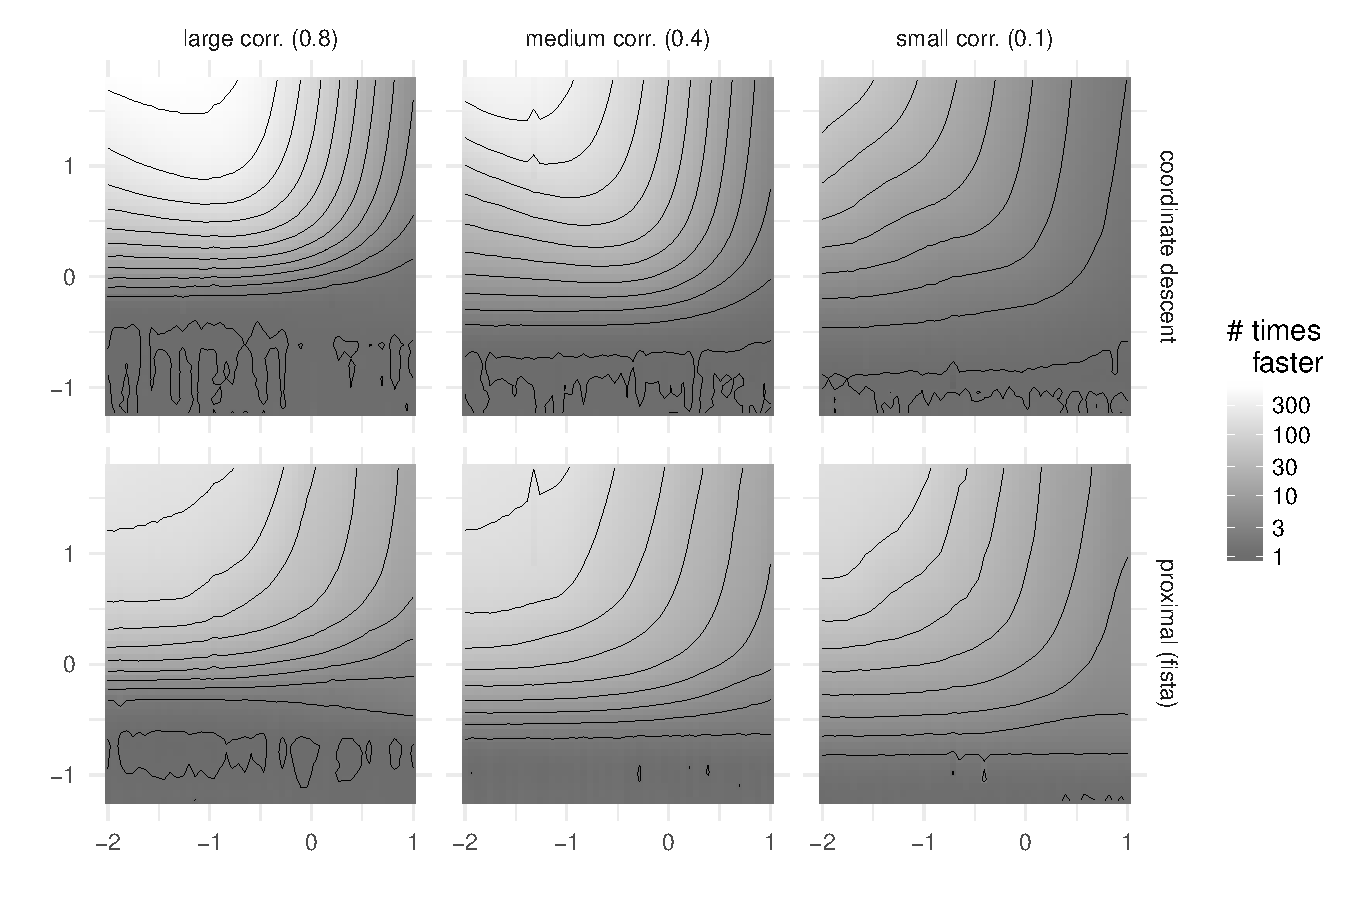
\includegraphics[angle=90,width=1.45\unitlength]{../figures/timing_all}}
      \put(1.45,1.65){\rotatebox{90.0}{\makebox[0cm]{$\log_{10}{\lambda_1}$}}}
      \put(1.45,1.05){\rotatebox{90.0}{\makebox[0cm]{$\log_{10}{\lambda_1}$}}}
      \put(1.45,0.45){\rotatebox{90.0}{\makebox[0cm]{$\log_{10}{\lambda_1}$}}}
      \put(0.4,0){\makebox[0cm]{$\log_{10}{\lambda_2}$}}
      \put(1.025,0){\makebox[0cm]{$\log_{10}{\lambda_2}$}}
%       \put(0,2.2){\line(1,0){1.5}}
    \end{picture} 
     \caption{Log-ratio of computation times for \mytexttt{coordinate} (left), and
     \mytexttt{proximal} (right), versus \mytexttt{quadratic}, for
     $(p,n)=(100,50),\, s=30$ and correlation $\rho \in \{0.1, 0.4, 0.8\}$
     (top, middle and bottom respectively).}
    \label{fig:timing_all}
  \end{figure}
\else
  \begin{figure}
    \centering
    \setlength{\unitlength}{0.5\linewidth}%
    \begin{picture}(2,1.2)%
      \put(0.025,0.025){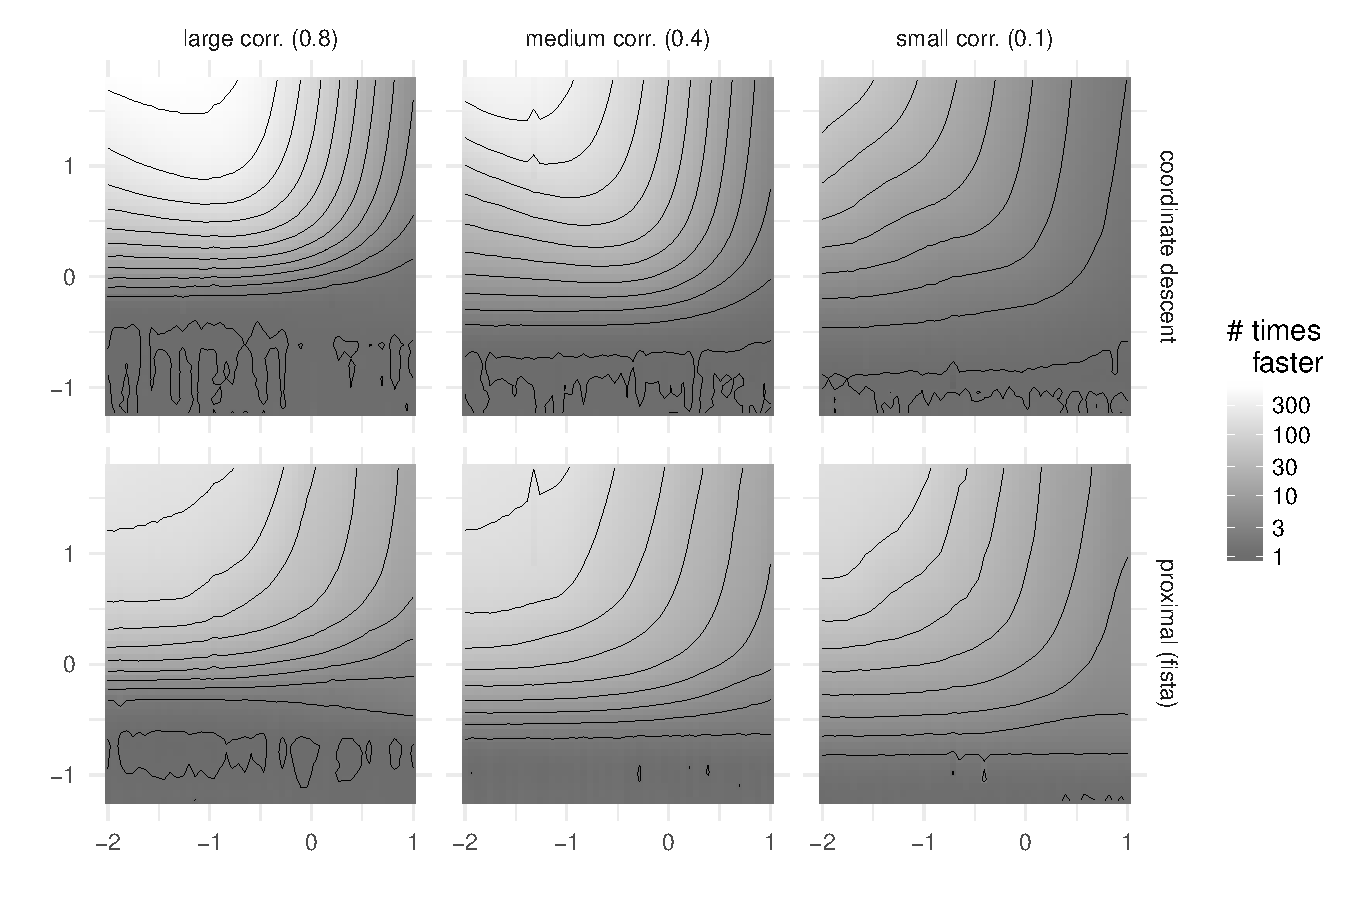
\includegraphics[angle=0,width=0.9\textwidth]{../figures/timing_all}}
      \put(0,0.4){\rotatebox{90.0}{\makebox[0cm]{$\log_{10}{\lambda_2}$}}}
      \put(0,0.9){\rotatebox{90.0}{\makebox[0cm]{$\log_{10}{\lambda_2}$}}}
      \put(0.45,0){\makebox[0cm]{$\log_{10}{\lambda_1}$}}
      \put(1,0){\makebox[0cm]{$\log_{10}{\lambda_1}$}}
      \put(1.45,0){\makebox[0cm]{$\log_{10}{\lambda_1}$}}
    \end{picture} 
     \caption{Log-ratio of computation times for \mytexttt{coordinate} (top) and
     \mytexttt{proximal} (bottom) versus \mytexttt{quadratic}, for high, medium
     and low variable correlation (left, center and right respectively).}
    \label{fig:timing_all}
  \end{figure}
\fi
Each map represents the log-ratio between the timing of either
\mytexttt{coordinate} or \mytexttt{proximal} versus \mytexttt{quadratic},
according to $(\lambda_1, \lambda_2)$ for a given correlation level.  
Dark regions with a value of 1 indicate identical running times while lighter
regions with a value of 10 indicate that \mytexttt{quadratic} is 10 times faster.
Figure~\ref{fig:timing_all} illustrates that \mytexttt{quadratic} outperforms both
\mytexttt{coordinate} and \mytexttt{proximal}, by running much faster in most
cases, even reaching 300-fold speed increases.  
The largest gains are observed for small $(\lambda_1,\lambda_2)$ penalty
parameters for which the problem is ill-conditioned, including many active
variables, resulting in a huge
slowdown of the first-order methods \mytexttt{coordinate} and
\mytexttt{proximal}.
As the penalty parameters increase, smaller gains are observed, especially when
$\lambda_2$, attached to the quadratic penalty, reaches high values for which all
problems are well-conditioned, and where the elastic net is leaning towards
univariate soft thresholding, in which case all algorithms behave similarly.

\iflong
  \subsection{Comparing Stand-Alone Implementations}
\fi

We  now  proceed  to the  evaluation  of  our  code with  three  other
stand-alone programs publicly  available as \mytexttt{R} packages.  We
chose     three    leading    state-of-the-art     packages,    namely
\mytexttt{glmnet}  \citep[Generalized  Linear  Models  regularized  by
Lasso    and    elastic-NET,][]{2009_JSS_Friedman},    \mytexttt{lars}
\citep[Least      Angle     Regression,     lasso      and     forward
Stagewise,][]{2004_AS_Efron}    and   \mytexttt{SPAMS}   \citep[SPArse
Modeling     Software,][]{2012_FML_Bach},     with     two     options
\mytexttt{SPAMS-FISTA},  which   implements  an  accelerated  proximal
method,   and  \mytexttt{SPAMS-LARS}   which   is  a   \mytexttt{lars}
substitute.   Note that  \mytexttt{glmnet} does  most of  its internal
computations  in \mytexttt{Fortran}, \mytexttt{lars}  in \mytexttt{R},
and  \mytexttt{SPAMS} in \mytexttt{C++}.   Our own  implementation, by
resolution  of the worst-case quadratic  problem,  is  shipped within  an
\mytexttt{R} package \mytexttt{quadrupen} publicly available at the second
author's        web         page\footnote{or        directly        at
  \mytexttt{\href{http://stat.genopole.cnrs.fr/logiciels/quadrupen}}. This
  will  be  made  available  on  the  CRAN  (Comprehensive  R  Archive
  Network)}.

We benchmark these packages by computing  regularization paths for the
Lasso\footnote{%
  We benchmark the packages on a Lasso problem since the parametrization of the
  elastic net problem differs among packages, hindering fair comparisons.},
that is, the elastic net Problem~\eqref{eq:enet} with $\lambda_2=0$.   
%
The inaccuracy of the solutions produced is measured by the gap in the objective
function compared to a reference solution, considered as being the true optimum.  
\iflong
  We use the \mytexttt{lars} solution as a reference, since it solves the Lasso problem
  up to the machine precision, relying on the \mytexttt{LAPACK/BLAS} routines. 
  % accessed via the \mytexttt{R} framework.
  Furthermore, \mytexttt{lars} provides the solution path for the Lasso,
  that is, the set of solutions computed for each penalty parameter value
  for which variable activation or deletion occurs, from the empty model to the
  least-mean squares model.
  This set of reference penalty parameters is used here to define a sensible reproducible choice.

  In high dimensional setups, the computational cost of returning the solutions
  for the largest models may be overwhelming compared to the one necessary
  for exploring the interesting part of the regularization path
  \citep{2011_JSS_Simon,2009_JSS_Friedman}.  This is mostly due to numerical
  instability problems that may be encountered in these extreme settings, where
  the Lasso solution is overfitting as it approaches the set of solutions to the
  underdetermined least squares problem.  We avoid a
  comparison mostly relying on these spurious cases by restricting the set
  of reference penalty parameters to the first $\min(n,p)$ steps of
  \mytexttt{lars} \citep[similar settings are used by][]{2009_JSS_Friedman}.

  Henceforth, the  distance $\mathrm{D}$  of a given  \mytexttt{method} to
  the optimum is evaluated on  the whole set of penalties $\Lambda$ used
  along the path, by
  \begin{equation*}
    \mathrm{D}(\mytexttt{method}) = \left( \frac{1}{|\Lambda|}\sum_{\lambda\in\Lambda}
      \left(J_{\lambda}^{\text{lasso}}\left(\hatbbeta_\lambda^{\mytexttt{lars}}\right)
        -J_{\lambda}^{\text{lasso}}\left(\hatbbeta_\lambda^{\mytexttt{method}}\right)\right)^2
       \right)^{1/2} 
    \enspace,
  \end{equation*}
  where $J_{\lambda}^{\text{lasso}}(\bfbeta) = J_{\lambda,0}^{\text{enet}}(\bfbeta)$ 
  is the objective function of the Lasso evaluated at $\bfbeta$, and
  $\hatbbeta_\lambda^{\mytexttt{method}}$ is the estimated optimal solution
  provided by the \mytexttt{method} package currently tested.
\fi

The data  sets are  generated according to  the linear  model described
above, in three different high-dimensional settings and small to medium number 
of variables: 
$(p,n)=(100,40)$, $(p,n)=(1\,000,200)$ and $(p,n)=(10\,000,400)$.  
The sparsity of the true underlying $\boldsymbol\beta^\star$ is governed by $s =
0.25\min(n,p)$, and the correlation between predictors is set by $\rho\in\{0.1, 0.4,  0.8\}$. For  each  value of
$\rho$, we averaged the timings over $50$ simulations, ensuring that each package
computes the solutions at identical $\lambda$ values, as defined above.

\iflong

  We pool together the runtimes obtained for the three levels of correlation for
  \mytexttt{quadrupen}, \mytexttt{SPAMS-LARS} and \mytexttt{lars}, which are not
  sensible to the correlation between features. 
  In each plot of Figure~\ref{fig:timing_glmnet}, each of these methods is thus 
  represented by a single point marking the average precision and the average distance to the
  optimum over the 150 runs (50 runs for each $\rho \in \{0.1, 0.4, 0.8\}$).
  Note that for \mytexttt{lars} only the abscissa is meaningful since
  $\mathrm{D}(\mytexttt{lars})$ is zero by definition.
  Besides, \mytexttt{quadrupen}, which solves each quadratic problem up to the
  machine precision, tends to be within this precision of the \mytexttt{lars}
  solution.%, as the required precision $\tau$ in \eqref{eq:tau_conv} was set here to $10^{-7}$.
  The \mytexttt{SPAMS-LARS} is also very precise, up to $10^{-6}$,
  which is the typical precision of the approximate resolution of linear systems.
  It is the fastest alternative for solving the Lasso when the problem is
  high-dimensional with a large number of variables (Figure
  \ref{fig:timing_glmnet}, bottom-left).

  \begin{figure}
    \centering
    \begin{tabular}{cc}
      \xylabelsquare{../figures/timing_others_low}{CPU time (in seconds, $\log_{10}$)}
                    {$\mathrm{D}(\mytexttt{method})$ ($\log_{10}$)}
                    {$n=100$, $p=40$}% 
      & \xylabelsquare{../figures/timing_others_med}{CPU time (in seconds, $\log_{10}$)}
                    {$\mathrm{D}(\mytexttt{method})$ ($\log_{10}$)}
                    {$n=200$, $p=1\,000$}% 
      \\[2ex] % 
      \xylabelsquare{../figures/timing_others_hig}{CPU time (in seconds, $\log_{10}$)}
                    {$\mathrm{D}(\mytexttt{method})$ ($\log_{10}$)}
                    {$n=400$, $p=10\,000$}% 
      & \xylabelsquare{../figures/timing_others_legend}{}{}{} \\
    \end{tabular}
    \caption{Distance  to optimum  versus CPU  time for  three different
     high-dimensional settings: $(p,n)=(100,40)$ (top left), $(p,n)=(1\,000,200)$
     (top right) and $p=(10\,000,400)$ (bottom left).  }
    \label{fig:timing_glmnet}
  \end{figure}

  In contrast, the (precision,timing)-values of \mytexttt{glmnet} and
  \mytexttt{SPAMS-FISTA} are highly affected by the threshold
  parameters\footnote{%
    In \mytexttt{glmnet}, convergence is monitored by the stability of the
    objective function, measured between two optimization steps, and
    optimization is halted when changes fall below the specified threshold
    (scaled by the null deviance).
    In \mytexttt{SPAMS-FISTA}, the stopping condition of the algorithm is based
    on the relative change of parameters between two iterations.}
  that control their stopping conditions.
  The computational burden to reach a given precision is also affected by the
  level of correlation, as illustrated in Figure~\ref{fig:timing_glmnet}.
  Obviously, a precise solution is difficult to reach with first-order descent
  algorithms in a high correlation setup, which corresponds to an
  ill-conditioned linear system.
  It may be surprising to observe that \mytexttt{SPAMS-FISTA} is about ten time
  slower than \mytexttt{glmnet}, as proximal and coordinate descent
  methods were experimentally shown to be roughly equivalent in our preceding
  analysis and by \citet{2012_FML_Bach}.
  However, these two comparisons were carried out with the same active set 
  strategy \citep[that is, \emph{with} active set for ours and \emph{without} 
  active set for][]{2012_FML_Bach}.
  We believe that this difference in the handling of active variables explains
  the relative bad performance of \mytexttt{SPAMS-FISTA}, which optimizes all
  variables along the regularization path, while  \mytexttt{glmnet} uses a 
  greedy active set strategy. 
%   Indeed, we observed a better match
%   between the performances of coordinate descent and accelerated proximal method
%   in our own implementations relying on the same active set strategy for all
%   approaches.

 Overall, our implementation is highly competitive, that is, very accurate, at
 the \mytexttt{lars} level, and much faster.  The speed improvements of
 \mytexttt{glmnet} are only observed for very rough approximate solutions and
 \mytexttt{SPAMS-FISTA} is dominated by \mytexttt{glmnet}. 
 Our experiments, in the framework of active set methods, agree with the results of
 \citet{2012_FML_Bach}: indeed, they observed that first-order methods are
 competitive with second-order ones only for low correlation levels and
 small penalties (which entails a large number of active variables).
 Conversely, our results may appear to contradict some of the experimental
 findings of \citet{2009_JSS_Friedman}: first, we observe that \mytexttt{glmnet}
 is quite sensitive to correlations, and second, the optimized second-order
 methods are competitive with \mytexttt{glmnet}.
 These differences in conclusions arise from the differences in experimental
 protocols: while we compare running times at a given accuracy, they are compared
 at a given threshold on the stopping criterion by \citet{2009_JSS_Friedman}.
 Regarding the influence of correlations, the stability-based criterion can be
 fooled due to the tiny step size that typically occurs for ill-conditioned
 problems, leading to a sizable early stopping.
 Regarding the second point, even though the \mytexttt{R} implementation of
 \mytexttt{lars} may indeed be slow compared to \mytexttt{glmnet}, considerable
 improvements can be obtained using optimized second-order methods such as 
 \mytexttt{quadrupen} as soon as a sensible accuracy is required, especially
 when correlation increases.
 
 Finally, among the accurate solvers, \mytexttt{SPAMS-LARS} is insignificantly
 less accurate than \mytexttt{quadrupen} or \mytexttt{lars} in a statistical
 context.  It is always faster than \mytexttt{lars} and slightly faster than
 \mytexttt{quadrupen} for the largest problem sizes (Figure
 \ref{fig:timing_glmnet}, bottom-left) and much slower for the smallest problem
 (Figure \ref{fig:timing_glmnet}, top-left).

%
\else
 The results, displayed in Figure  \ref{fig:timing_glmnet}, show that our
 implementation is highly competitive, that is, very accurate, at the \mytexttt{lars} 
 level, and much faster.  The speed improvements of \mytexttt{glmnet} 
 are only observed for very rough approximate solutions and
 \mytexttt{SPAMS} FISTA is dominated by \mytexttt{glmnet}.
  Finally, \mytexttt{SPAMS} homotopy is slightly less accurate than
  \mytexttt{quadrupen}  and \mytexttt{LARS} but  it is the fastest accurate
  alternative for the largest problem sizes (Figure  \ref{fig:timing_glmnet}, right). 

  \begin{figure}
    \centering 
    \begin{tabular}{@{}c@{}c@{}c@{}c@{}}
      \xylabelsquare{../figures/timing_others_low}{CPU     time
        ($\log_{10}$)}{optimization gap ($\log_{10}$)}{}% 
      & \xylabelsquare{../figures/timing_others_med}{CPU time
        ($\log_{10}$)}{}{} % 
      \xylabelsquare{../figures/timing_others_hig}{CPU     time
        ($\log_{10}$)}{}{}%
      & \xylabelsquare{../figures/timing_others_legend}{}{}{} \\
    \end{tabular}
    \caption{Distance  to optimum  versus CPU  time for  three different
     high-dimensional settings: $p=100,\ n=40$ (left), $p=1\,000,\
     n=200$ (center) and
     $p=10\,000,\ n=400$ (right). }
    \label{fig:timing_glmnet}
  \end{figure}
\fi





\subsection{Link between accuracy of solutions and prediction performances}
\label{sec:fromatop}

When the ``irrepresentable condition'' \citep{2006_JMLR_Zhao} holds, the
Lasso should  select the true model consistently.   However, even when
this  rather  restrictive  condition  is  fulfilled,  perfect  support
recovery  obviously requires numerical  accuracy:
rough estimates may speed up the procedure, but whatever optimization strategy
is used, stopping an algorithm is likely to prevent either the removal of all
irrelevant coefficients or the insertion of all relevant ones.  The support of 
the solution may then be far from the optimal one. 

We  advocate here  that our  quadratic solver  is very  competitive in
computation time when support recovery matters, that is, when high level  of accuracy is needed, in small (few
hundreds of variables) and  medium sized problems (few thousands).  As
an  illustration,  we  
% highlight  a  simple  situation  where  such  a
% desideratum arises:  we 
generate 100 data sets under the linear model described above, with a rather
strong coefficient of determination ($R^2
\approx 0.8$ on  average), a rather high level  of correlation between
predictors ($\rho=0.8$) and a medium level of sparsity ($s/p = 30\%$).
The number of  variable is kept low ($p=100$) and  the difficulty of the
estimation problem  is tuned  by the  $n/p$  ratio. For  each data  set, we  also
generate a  test set sufficiently  large (say, $10n$) to  evaluate the
quality of the prediction without  depending on any sampling fluctuation.  
We compare the Lasso solutions computed by \mytexttt{quadrupen} to the ones returned by
\mytexttt{glmnet} with
various   level   of    accuracy\footnote{This   is   done   via   the
  \mytexttt{thresh}  argument of  the  \mytexttt{glmnet} procedure,  whose
  default  value  is \mytexttt{1e-7}.   In  our  experiments,
  \mytexttt{low}, \mytexttt{med}  and \mytexttt{high}  level of  accuracy for
  \mytexttt{glmnet} respectively correspond to \mytexttt{thresh} set to
  \mytexttt{1e-1}, \mytexttt{1e-4}, and \mytexttt{1e-9}.}.  
Figure \ref{fig:accuracy} reports performances, as measured by the mean squared
test error and the support error rate.

\begin{figure}[htbp]
  \centering
  \begin{tabular}{@{}l@{}c@{}} 
    \rotatebox{90.0}{\makebox[.6\textwidth]{\hspace{.3\textwidth} Support Error 
    Rate \hspace{.35\textwidth} MSE}}
    &
    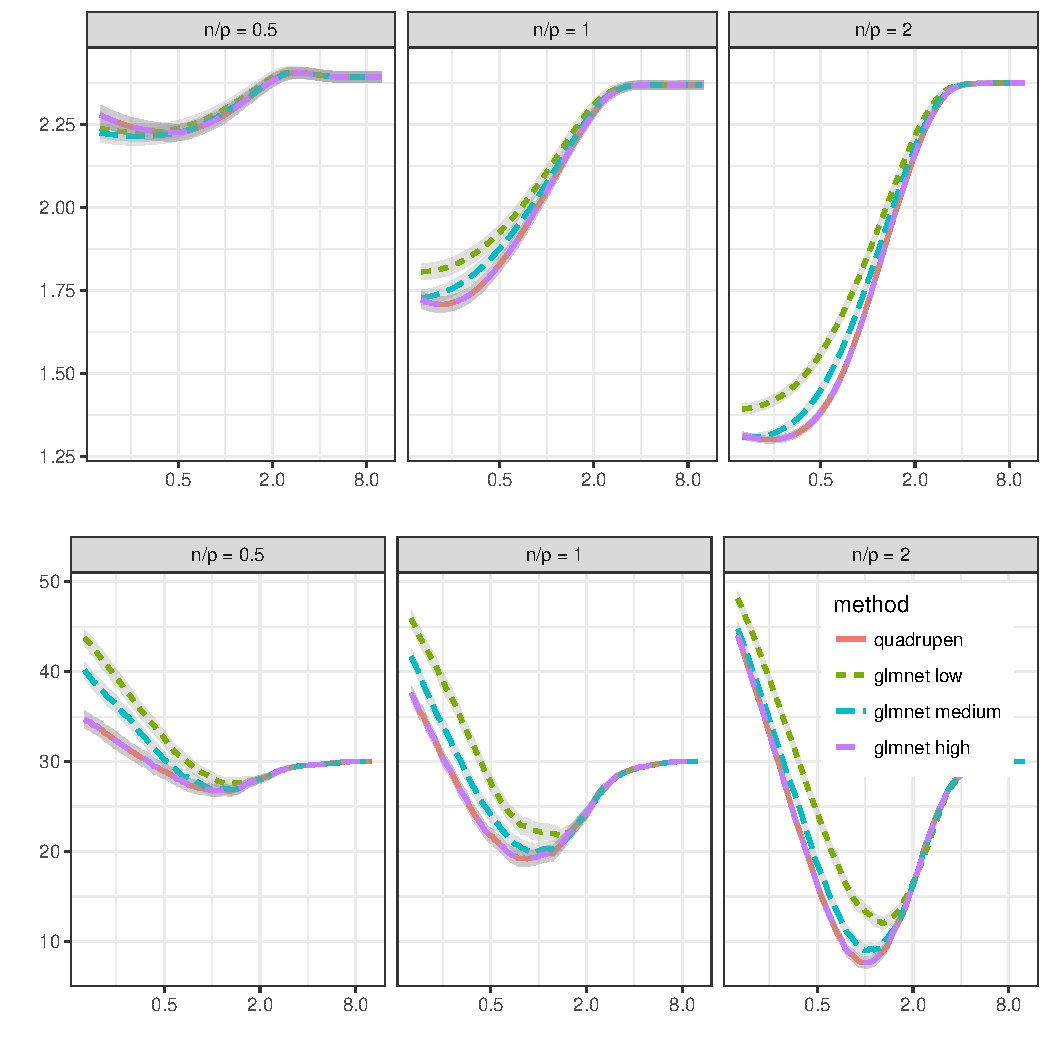
\includegraphics[angle=0,width=\textwidth]{../figures/accuracy}
  \end{tabular}
  \caption{Test performances according to the penalty parameter for the
    Lasso estimates returned by \mytexttt{quadrupen} and \mytexttt{glmnet} at various level
    of accuracy. Three high-dimensional setups are illustrated: from left to 
    right $n/p=1/2$, $n/p=1$ and $n/p=2$;
    top: mean squared test error;
    bottom: support error rate.\label{fig:accuracy}}
\end{figure} 

As expected, the curves show that selecting variables and searching for
the best prediction are two different problems.  The selection problem
(bottom  of Figure \ref{fig:accuracy}) always  requires a sparser  model than the
prediction  problem.  But  despite this  obvious difference,  the more
accurate the solution returned by the algorithm, the better  the performances for any levels of
penalty and for  both performance measures. 
% Regarding  the MSE though (upper
% part of  the Figure), an interesting  point concerns the  shape of the
% error  curve: a  high level  of accuracy  tends to  produce  less flat
% curves with clearer  minimums, which may have an  important impact for
% model selection.   This question is of particular  interest for penalized
% procedures such as the Lasso, where the choice of the tuning parameter
% remains a bottleneck commonly dealt with cross-validation.

\begin{table}[htbp]

  \begin{tabular}{@{}l|cccc@{}}
    methods & \mytexttt{quadrupen} & \mytexttt{glmnet\,low} & \mytexttt{glmnet\,med} & \mytexttt{glmnet\,high} \\
    \hline
    timing (ms) & 8 & 7 & 8 & 64 \\
    accuracy (dist.  to opt.)  & $5.9\times 10^{-14}$ & $7.2 \times 10^{0}$ & $6.04 \times 10^{0}$ & $1.47 \times 10^{-2}$\\
  \end{tabular}
  \caption{Median timings and solution accuracies% for the experiments
                                % of Section~\ref{sec:fromatop}.
  }
  \label{tab:accuracy}
\end{table} 

Now focusing on \mytexttt{glmnet} performances, the better the accuracy,
the  smaller the  MSE  and the  support  error rate.  But  the better  the
accuracy,  the  slower  the  algorithm  becomes.   Using  the  default
settings allows to have a result very close to our quadratic solver, and the
performance differences become negligible between our approach and \mytexttt{glmnet}
running with high precision.
However, Table \ref{tab:accuracy} illustrates that high accuracy is achieved at 
a high computational cost: to be at par with \mytexttt{quadrupen} with regards to
test performances, \mytexttt{glmnet} is about ten times slower than our solver.





